
\section{Parameter tuning}

\Warning[TODO]{ Combine into algorithm comparison! }


\subsection{katz-eig}

There are two parameters to \textit{katz-eig}: $\beta$, the link diminishing factor and $K$ specifying the $K$-rank approximation. $\beta$ is a continous value satisfying $0 < \beta \leq \frac{1}{\|A_{train}\|_2}$. If $\beta = 0$ then the algorithm will only output 0 and if $\beta > \frac{1}{\|A_{train}\|_2}$ the iterations will not converge. $K > 0$ is a discrete value.

What follows is plots over both of the parameters $K$ and $\beta$. The plots are evaluated using \textit{F-measure} w.r.t. the test set using top-10 recommendations.

\begin{figure}[h!]
\centering
\begin{minipage}{.5\textwidth}
    \centering
    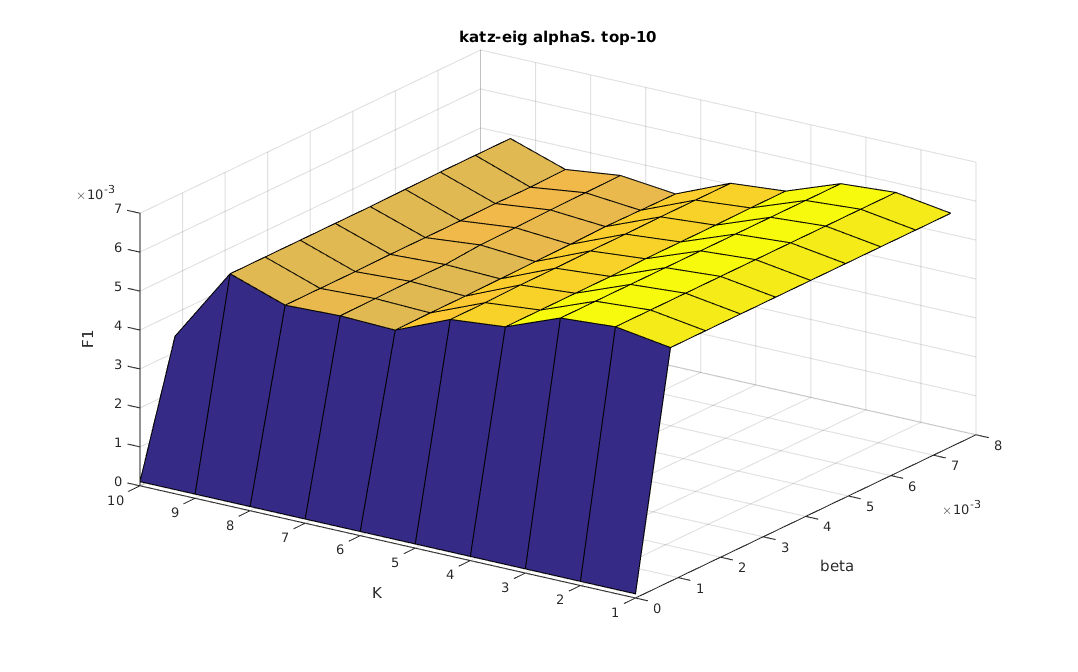
\includegraphics[width=\linewidth]{fig/katzeig_beta_k/alphaS_katzeig.png}
    \captionof{figure}{\textit{alphaS}}
\end{minipage}%
\begin{minipage}{.5\textwidth}
    \centering
    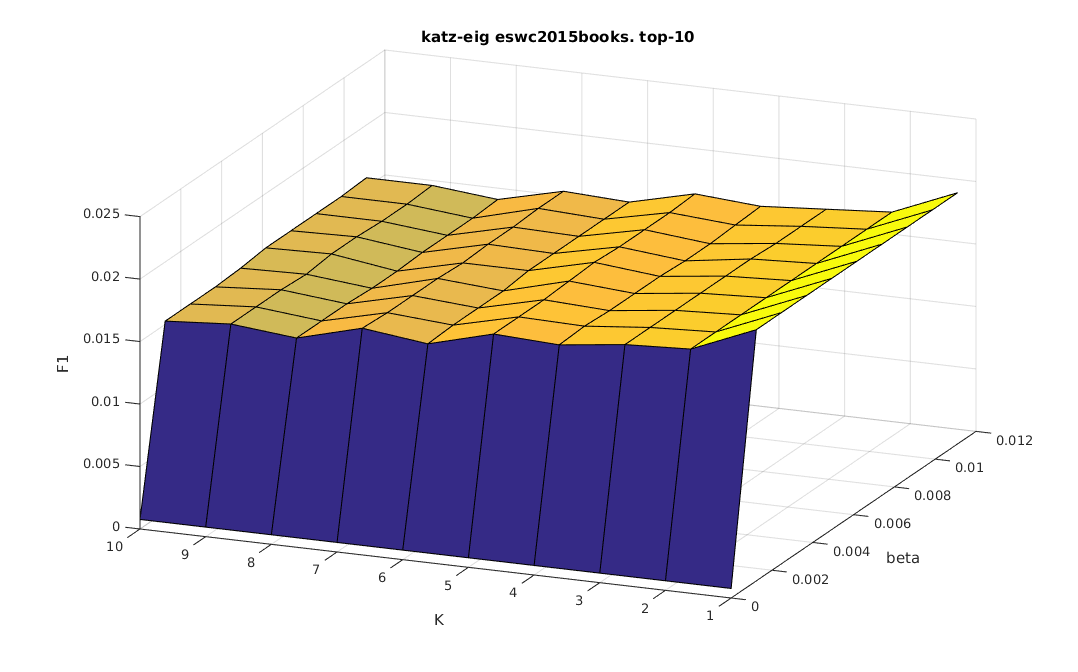
\includegraphics[width=\linewidth]{fig/katzeig_beta_k/eswc2015books_katzeig.png}
    \captionof{figure}{\textit{eswc2015books}}
\end{minipage}
\end{figure}

\begin{figure}[h!]
\centering
\begin{minipage}{.5\textwidth}
    \centering
    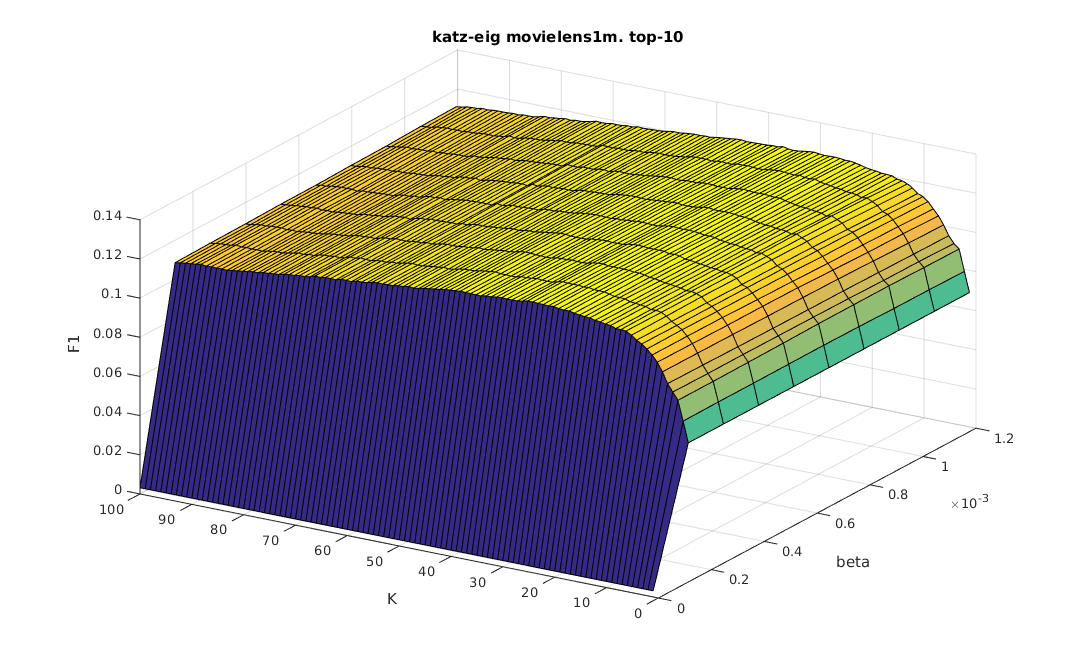
\includegraphics[width=\linewidth]{fig/katzeig_beta_k/movielens_katzeig.png}
    \captionof{figure}{\textit{movielens1m}}
\end{minipage}%
\begin{minipage}{.5\textwidth}
    \centering
    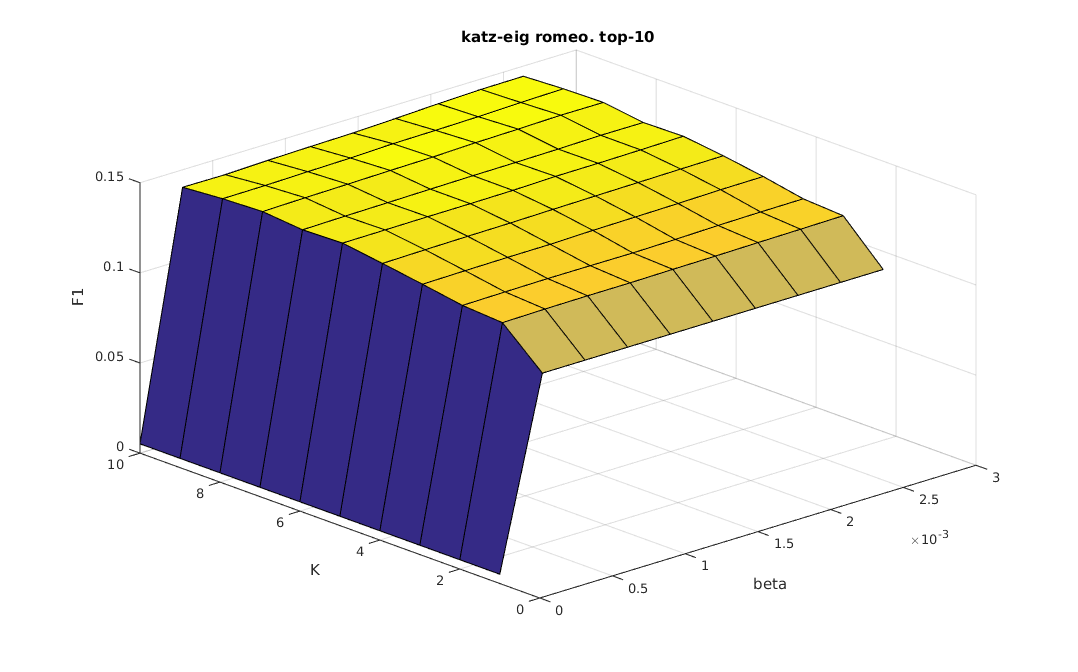
\includegraphics[width=\linewidth]{fig/katzeig_beta_k/romeo_katzeig.png}
    \captionof{figure}{\textit{romeo}}
\end{minipage}
\end{figure}




It seems like $beta$ doesn't have a very big impact on the function value. Some plots with a fixed $K$ follows to better see differences.

The range examined is $0 < \beta \leq \beta_{max} = \frac{1}{\|A_{train}\|_2}$ with a $K$ selected to fit the specific dataset. Again evaluated using \textit{Precision}, \textit{Recall} and \textit{F-measure} w.r.t. the test set using the top-10 recommendations.

\FloatBarrier

\begin{figure}[h!]
\centering
\begin{minipage}{.5\textwidth}
    \centering
    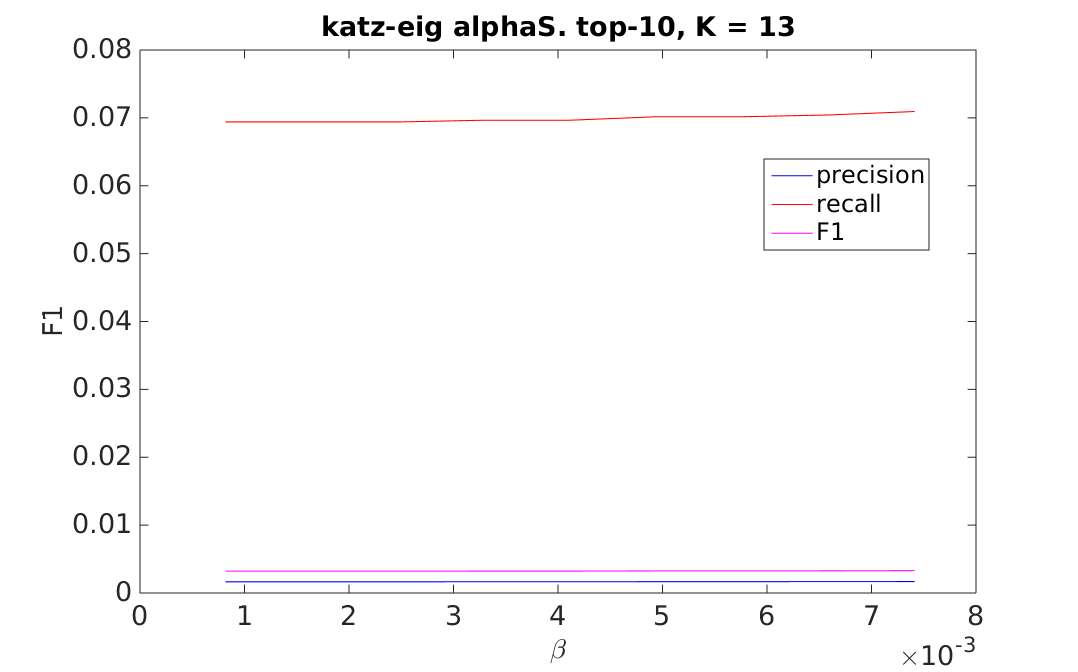
\includegraphics[width=\linewidth]{fig/katzeig_beta/alphaS_katzeig_beta.png}
    \captionof{figure}{\textit{alphaS}.
        $\beta_{max}$ is the best value with a $1.9\%$ diff between the minimum and the maximum \textit{F1} value.}
\end{minipage}%
\begin{minipage}{.5\textwidth}
    \centering
    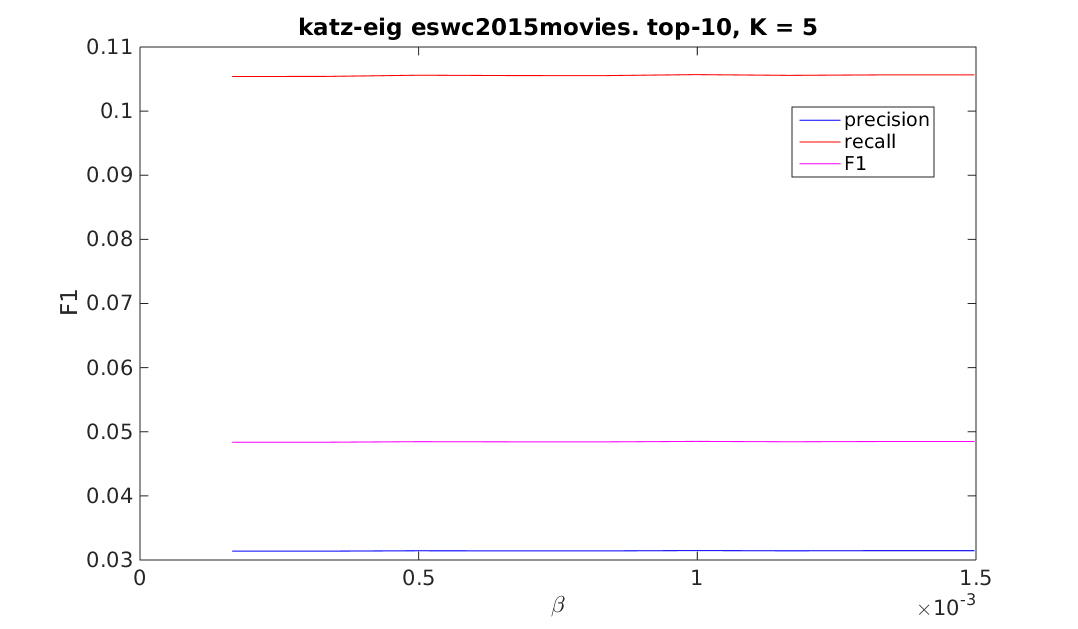
\includegraphics[width=\linewidth]{fig/katzeig_beta/eswc2015movies_katzeig_beta.png}
    \captionof{figure}{\textit{eswc2015movies}.
        $\beta_{max}$ is not the best value with a $0.3\%$ diff between the minimum and the maximum \textit{F1} value.}
\end{minipage}
\end{figure}

\begin{figure}[h!]
\centering
\begin{minipage}{.5\textwidth}
    \centering
    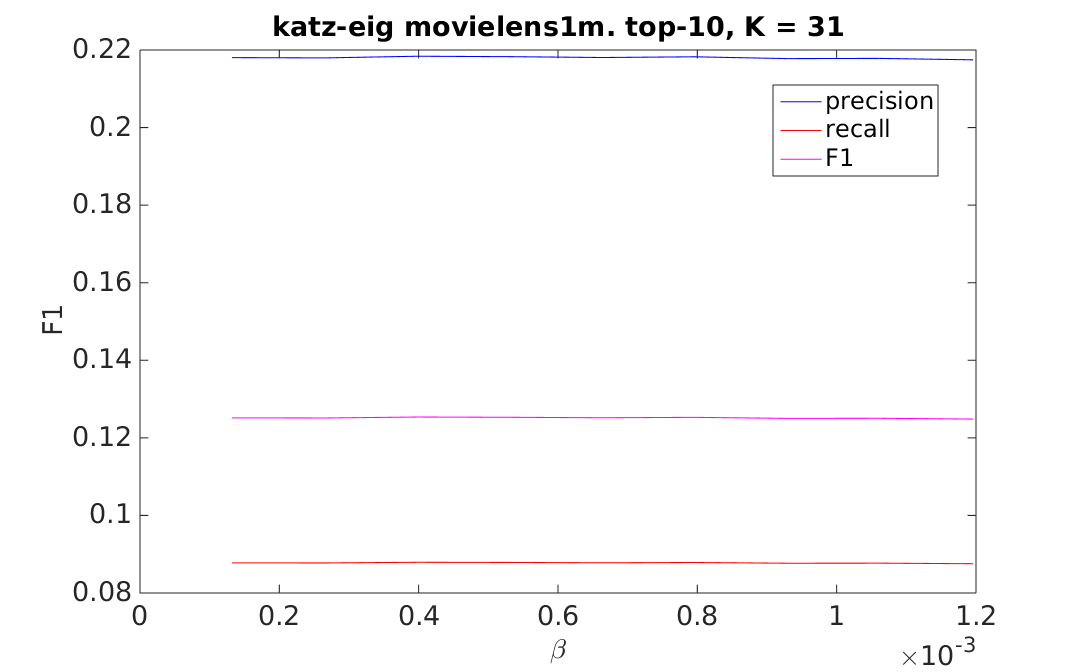
\includegraphics[width=\linewidth]{fig/katzeig_beta/movielens_katzeig_beta.png}
    \captionof{figure}{\textit{movielens1m}.
        $\beta_{max}$ is not the best value with a $0.41\%$ diff between the minimum and the maximum \textit{F1} value.}
\end{minipage}%
\begin{minipage}{.5\textwidth}
    \centering
    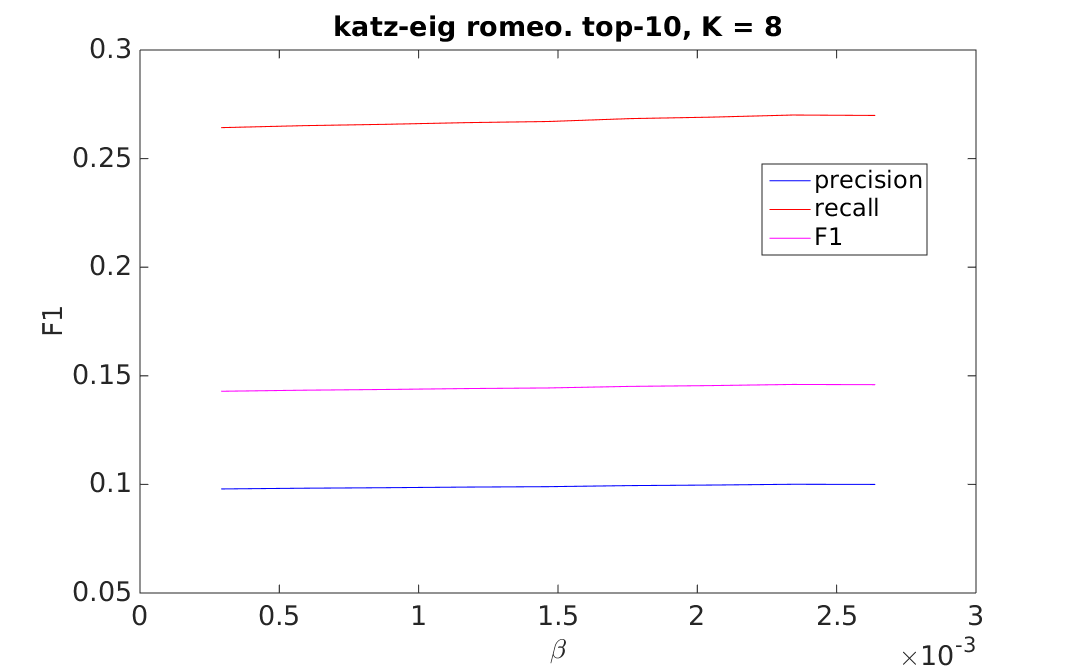
\includegraphics[width=\linewidth]{fig/katzeig_beta/romeo_katzeig_beta.png}
    \captionof{figure}{\textit{movielens1m}.
        $\beta_{max}$ is not the best value with a $2.09\%$ diff between the minimum and the maximum \textit{F1} value.}
\end{minipage}
\end{figure}

\FloatBarrier

The difference between the optimal $\beta$ and an arbitrary selected $\beta$ isn't very large. Even smaller is the difference between the optimal $\beta$ and $\beta_{max}$.  \Tableref{tab:katzeig_beta} is a summary of the evaluated values.

\begin{table}[h!]
    \centering
    \begin{tabular}{| c | r | r | r | r | l |}
        \hline
        \textbf{dataset}        & \textbf{diff between $\beta_{opt}$ and $\beta_{max}$ }    & \textbf{diff between $f_{min}$ and $f_{max}$} \\ \hline

        \textit{alphaS}         & 0~\%      & 2.0~\%    \\ \hline
        \textit{eswc2015books}  & 0~\%      & 0\%       \\ \hline
        \textit{eswc2015movies} & 0.039~\%  & 0.28~\%   \\ \hline
        \textit{movielens1m}    & 0.41~\%   & 0.41~\%   \\ \hline
        \textit{romeo}          & 0.072~\%  & 2.1~\%    \\ \hline


    \end{tabular}
    \caption{A summary of evaluating different $\beta$. $\beta_{max} = \frac{1}{\|A_{train}\|_2}$ is the maximally examined $\beta$ and $\beta_{opt}$ is the optimal $\beta$ found in the range $0 < \beta \leq \beta_{max}$. $K$ is individually optimized for the different datasets. $f_{min}$ and $f_{max}$ are the minimal and maximal \textit{F1} values obtained.}
    \label{tab:katzeig_beta}
\end{table}

\FloatBarrier

\newpage


The $K$-rank approximation represents different available models for \textit{katz-eig}. The following plots show different values of $K$, evaluated w.r.t. the test set. $\beta = \frac{1}{\|A_{train}\|}_2$ for all datasets. $K_{m}$ is the value of $K$ which gives the best \textit{F-measure} for each dataset.

\FloatBarrier

\begin{figure}[h!]
\centering
\begin{minipage}{.5\textwidth}
    \centering
    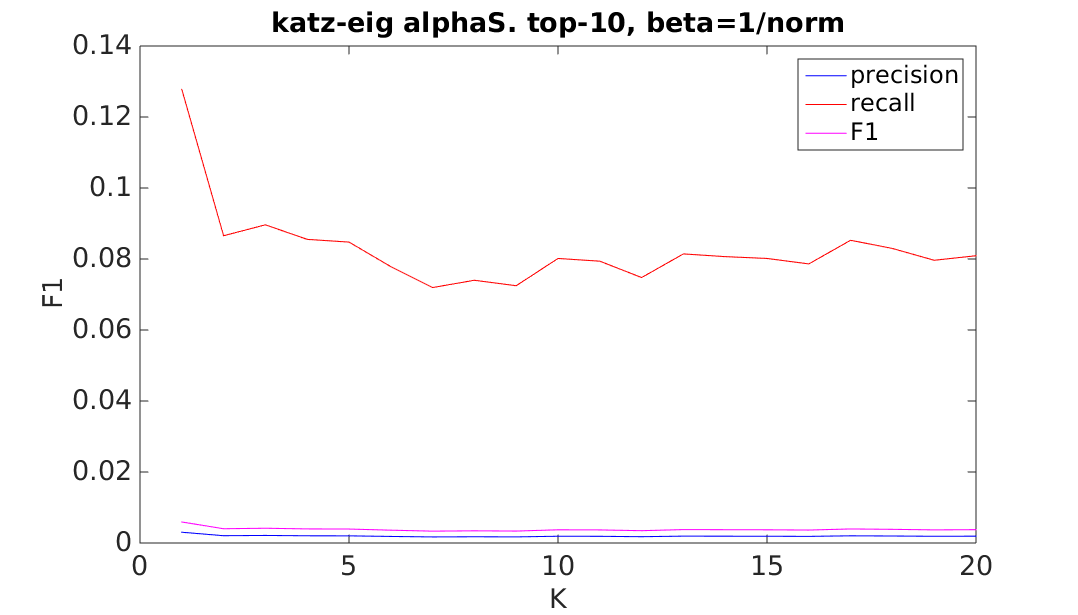
\includegraphics[width=\linewidth]{fig/katzeig_k/alphaS_katzeig_K.png}
    \captionof{figure}{\textit{alphaS} $K_{m} = 13$}
\end{minipage}%
\begin{minipage}{.5\textwidth}
    \centering
    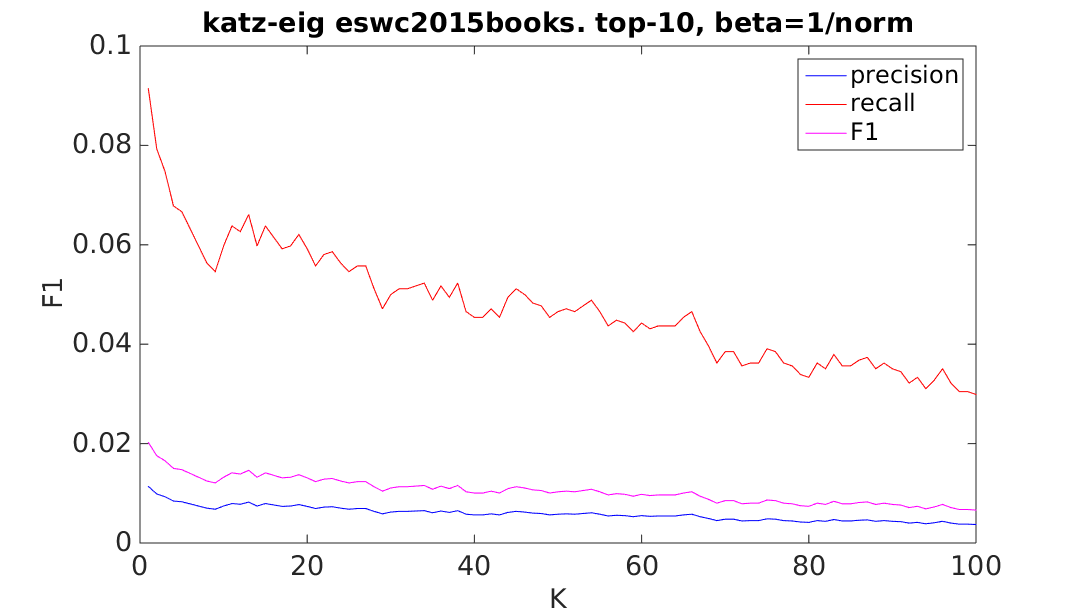
\includegraphics[width=\linewidth]{fig/katzeig_k/eswc2015books_katzeig_K.png}
    \captionof{figure}{\textit{eswc2015books} $K_{m} = 1$}
\end{minipage}
\end{figure}

\begin{figure}[h!]
\centering
\begin{minipage}{.5\textwidth}
    \centering
    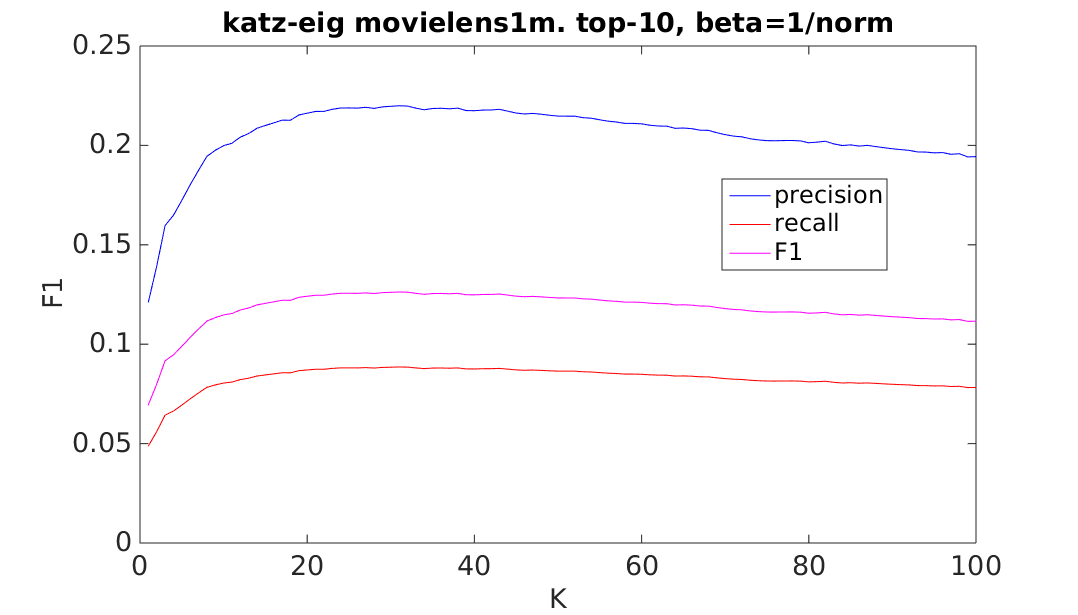
\includegraphics[width=\linewidth]{fig/katzeig_k/movielens_katzeig_K.png}
    \captionof{figure}{\textit{movielens1m} $K_{m} = 31$}
\end{minipage}%
\begin{minipage}{.5\textwidth}
    \centering
    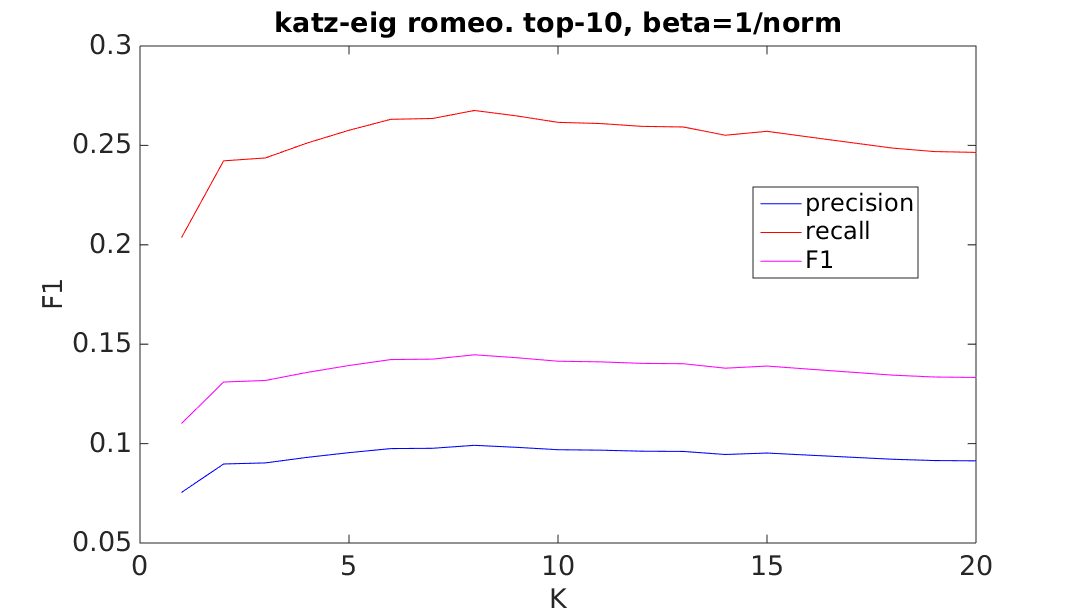
\includegraphics[width=\linewidth]{fig/katzeig_k/romeo_katzeig_K.png}
    \captionof{figure}{\textit{romeo} $K_{m} = 8$}
\end{minipage}
\end{figure}

\Warning[TODO]{ Plot of \textit{eswc2015movies}? }

%\begin{figure}[h!]
%\centering
%\begin{minipage}{.5\textwidth}
    %\centering
    %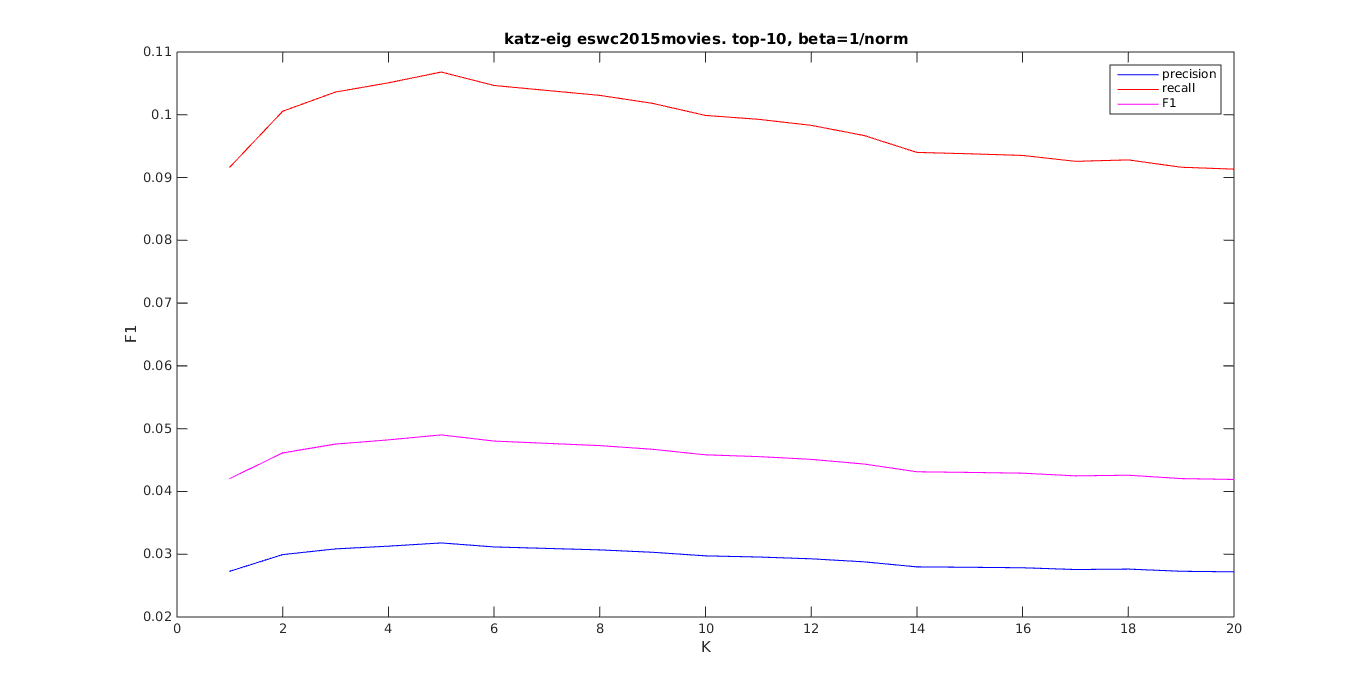
\includegraphics[width=\linewidth]{fig/katzeig_k/eswc2015movies_katzeig_K.png}
    %\captionof{figure}{\textit{eswc2015movies} $K_{m} = 5$}
%\end{minipage}%
%\begin{minipage}{.5\textwidth}
    %\centering
    %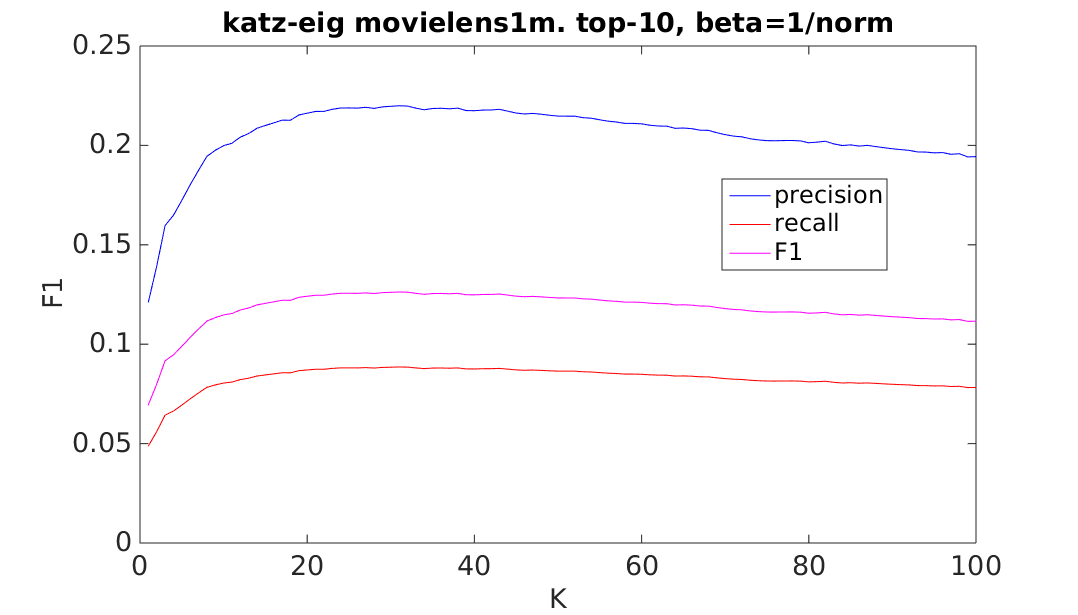
\includegraphics[width=\linewidth]{fig/katzeig_k/movielens_katzeig_K.png}
    %\captionof{figure}{\textit{movielens1m} $K_{m} = 31$}
%\end{minipage}
%\end{figure}

%\begin{figure}[h!]
%%\centering
%\begin{minipage}{.5\textwidth}
    %%\centering
    %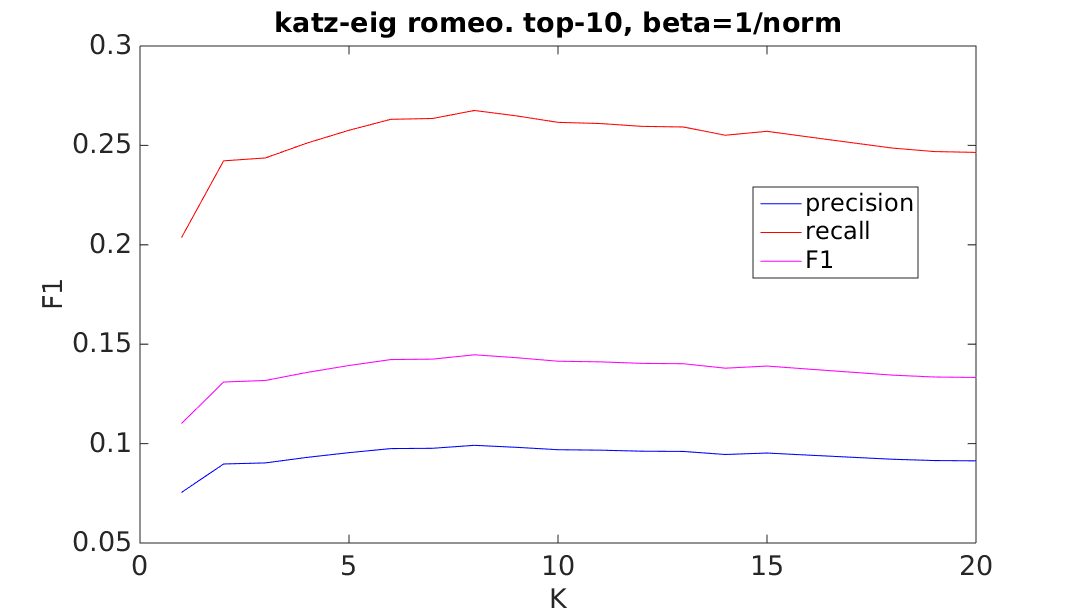
\includegraphics[width=\linewidth]{fig/katzeig_k/romeo_katzeig_K.png}
    %\captionof{figure}{\textit{romeo} $K_{m} = 8$}
%\end{minipage}%
%\end{figure}

\FloatBarrier

The function space w.r.t. $K$ is fairly smooth if not entirely convex. \textit{eswc2015books} is an outlier with a low optimal value $K = 1$ and many local optima. The other datasets display more smooth functions, but there are clear local optima with both \textit{alphaS} and \textit{romeo}.

Also of note is that the functions start to decline at different $K$. \textit{eswc2015movies} declines already at $K = 5$ but it's only at around $K = 30$ \textit{movielens1m} starts to decline. As noted earlier \textit{eswc2015books} has it's optima already at $K = 1$.


\newpage

\section{The link-analysis algorithm}\label{sec:linkanalysis}

%\textit{Cleanup, mostly description from article. Reduce information?}

The \textit{link-analysis} algorithm, as presented by \cite{huang2004link} and further discussed in \cite{huang2007comparison}. See the articles for more information and in-depth examples. What follows is a condensed description of how the algorithm works.

The algorithm is an adaptation of HITS \cite{kleinberg1999authoritative} which is a web page ranking algorithm to the recommendation domain. The original algorithm distinguish between \textit{Authoritative} pages which definitely contain high-quality information and \textit{Hub} pages which are comprehensive lists of links to authoritative pages. \citep{huang2007comparison}

The adaptation to the recommendation domain is achieved by introducing the \textit{product representativeness} score $\PR$ and the \textit{consumer representativeness} score $\CR$.

The \textit{product representativeness} score $\PR(i, u)$ can be seen as a measure of the item $i$'s level of interest with respect to user $u$, or in other words $i$'s authority of $u$'s interests in $i$.

The \textit{consumer representativeness} score $\CR(u, \hat{u})$ measures how well $u$ as a hub for $\hat{u}$ associates with products of interests to $\hat{u}$.

If $h_{u, i}$ is the user-item interaction history as defined by \ref{eq:hist} and $h$ is the interaction matrix then a recursive definition of the authority and hub scores can be defined as

\begin{equation}
    \PR = h' * \CR
\end{equation}

\begin{equation}
    \CR = B * \PR + \CR_0
\end{equation}

Where $B$ is a matrix such that:

\begin{equation}
    B_{u, i} = \frac{ h_{u, i} }{ \left(\sum_{i} h_{u, i}\right)^\gamma }
\end{equation}

Meaning $B$ normalizes the representativeness score a costumer receives from linked products by dividing it with the total number of products the customer is linked to.  $\gamma$ controls the extent to which a consumer is penalized for making many purchases.

$\CR_0$ is defined as

\begin{equation}
    \CR_{i, j}^0 = \begin{cases}
        \eta \quad \text{if } \; i = j \\
        0    \quad \text{otherwise}
    \end{cases}
\end{equation}

in other words $\CR_0 = \eta * I_M$ where $I_M$ is an $M x M$ identity matrix and $M$ is the number of users.  It is included to maintain the high representativeness score for the target users themselves. This also necessitates a normalization step to keep the values on a consistent level.

In summary the \textit{link-analysis} algorithm follow these steps:

\begin{enumerate}
    \item Construct the interaction matrix $A$ and the associating matrix $B$.

    \item Set $\CR_0 = \eta * I_M$.
    \item At each iteration $t = 1, \ldots, t_{max}$ perform:

        \begin{enumerate}
            \item $\PR_t = h' * \CR_{t- 1}$
            \item $\CR_t = B * \PR_t$
            \item Normalize $\CR_t$ so each column adds up to 1
            \item $\CR_t = \CR_t + \CR_0$
        \end{enumerate}

        Repeat until convergence.

    \item Predicted user-item interaction is given by $\mathit{pval} = \PR'$.

\end{enumerate}

There are two parameters to the algorithm: $\gamma$ and $\eta$.
%\Warning[TODO]{ Describe them, what's their purpose }


\newpage


\section{Algorithm comparison}


\Warning[TODO]{ Compare with a simple top-list? Or something else easy? }

\begin{enumerate}
    \item Time to optimize for different datasets
    \item Time to recommend given optimized parameters
    \item Performance of recommendations given optimized parameters
\end{enumerate}

\begin{table}[h!]
    \centering
    \begin{tabular}{| c | c | c | c | c |}
        \hline
        \textbf{}               & \multicolumn{2}{c|}{\textbf{katz-eig}} & \multicolumn{2}{c|}{\textbf{link-analysis}} \\ \hline
        \textit{alphaS}         & 41.876401     & 9.106161         & 26.978338     & 0.877453      \\ \hline
        \textit{eswc2015books}  & 1.871681      & 0.023562         & 3.245297      & 0.026975      \\ \hline
        \textit{eswc2015movies} & 52.749416     & 5.194185         & x             & x             \\ \hline
        \textit{eswc2015music}  & 141.664568    & 5.769257         & x             & x             \\ \hline
        \textit{movielens1m}    & 31.249456     & 0.190485         & 244.484291    & 58.205089     \\ \hline
        \textit{romeo}          & 3.781222      & 0.012321         & 81.478788     & 4.675901      \\ \hline
    \end{tabular}
    \caption{Runtime for optimizing the different algorithms for the different datasets. Uses the fastest optimization strategy.}
    \label{tab:alg_full_time}
\end{table}

\begin{table}[h!]
    \centering
    \begin{tabular}{| c | c | c | c | c |}
        \hline
        \textbf{}               & \multicolumn{2}{c|}{\textbf{katz-eig}} & \multicolumn{2}{c|}{\textbf{link-analysis}} \\ \hline
        \textit{alphaS}         & 3.434409 s & 1.038829 & 10.307018 s  & 0.068634       \\ \hline
        \textit{eswc2015books}  & 0.027989 s & 0.004293 & 0.720686 s   & 0.016339       \\ \hline
        \textit{eswc2015movies} & 1.382029 s & 0.516727 & x            & x              \\ \hline
        \textit{eswc2015music}  & 2.001985 s & 0.159226 & x            & x              \\ \hline
        \textit{movielens1m}    & 1.410586 s & 0.107071 & 154.404908 s & 18.179708      \\ \hline
        \textit{romeo}          & 0.216897 s & 0.032052 & 40.477119 s  & 0.114363       \\ \hline
    \end{tabular}
    \caption{Runtime of the algorithms using the full interaction history using the optimized parameters given in \appendixref{app:opt_params}.}
    \label{tab:alg_full_time}
\end{table}


\begin{table}[h!]
    \centering
    \begin{tabular}{| c | c | c | }
        \hline
        \textbf{}               & \textbf{katz-eig} & \textbf{link-analysis} \\ \hline
        \textit{alphaS}         & 0.002174          & \textbf{0.003208}      \\ \hline
        \textit{eswc2015books}  & 0.020102          & \textbf{0.023537}      \\ \hline
        \textit{eswc2015movies} & \textbf{0.048456} & x                      \\ \hline
        \textit{eswc2015music}  & \textbf{0.054448} & x                      \\ \hline
        \textit{movielens1m}    & \textbf{0.124839} & 0.090044               \\ \hline
        \textit{romeo}          & \textbf{0.145914} & 0.134655               \\ \hline
    \end{tabular}
    \caption{Performance on \textit{F-measure} of the different algorithms using the optimized parameters given in \appendixref{app:opt_params}.}
    \label{tab:alg_full_perf}
\end{table}

%\begin{figure}[h!]
    %\centering
    %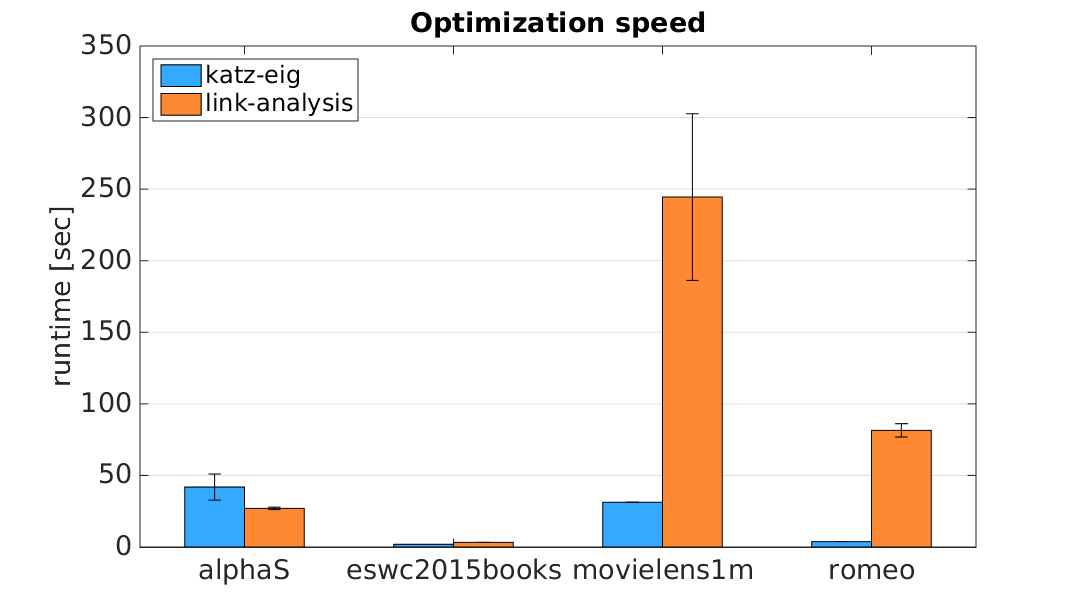
\includegraphics[width=0.9\textwidth]{fig/comp/comp_rec_opt_time.png}
    %\caption{totod}
%\end{figure}

\begin{figure}[h!]
    \begin{subfigure}[h!]{0.5\textwidth}
        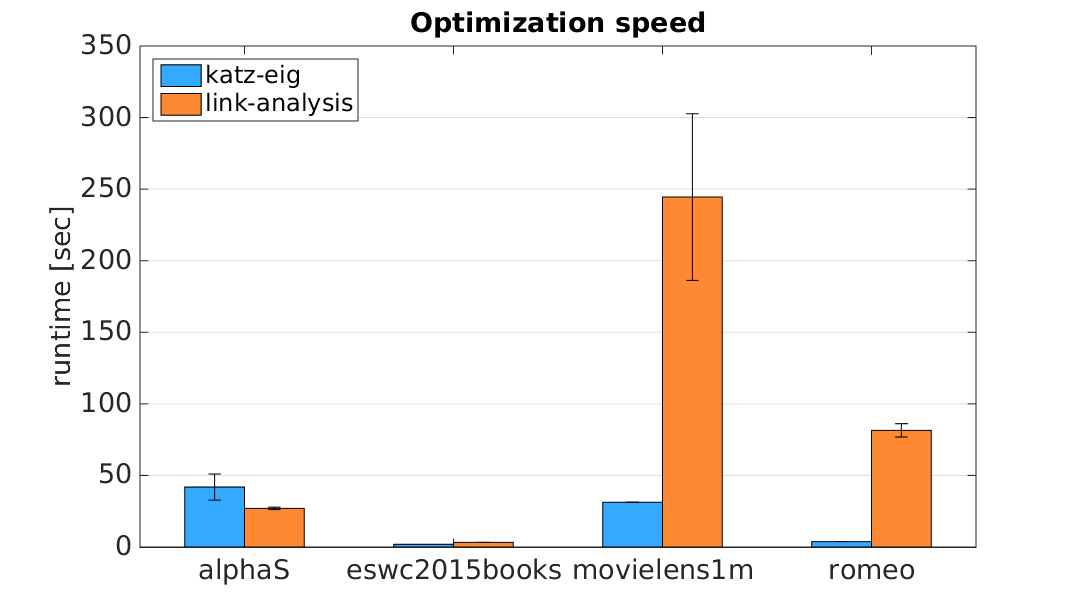
\includegraphics[width=\textwidth]{fig/comp/comp_rec_opt_time.png}
        \caption{}
        %\label{fig:rec_speed}
    \end{subfigure}
    ~
    \begin{subfigure}[h!]{0.5\textwidth}
        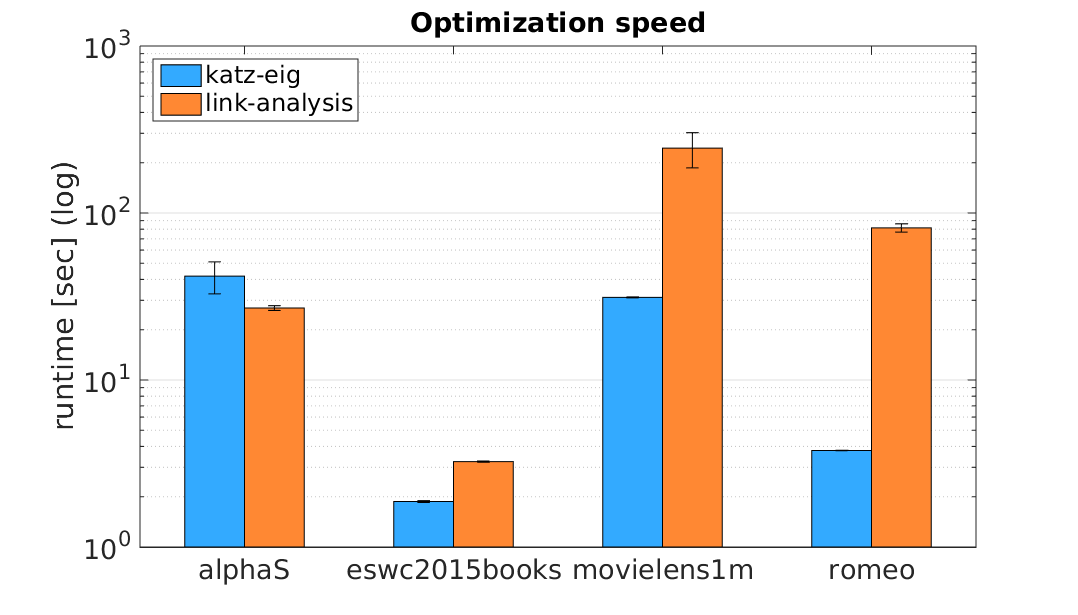
\includegraphics[width=\textwidth]{fig/comp/comp_rec_opt_time_log.png}
        \caption{}
        %\label{fig:rec_speed_log}
    \end{subfigure}
    \caption{TODO}
\end{figure}

\begin{figure}[h!]
    \centering
    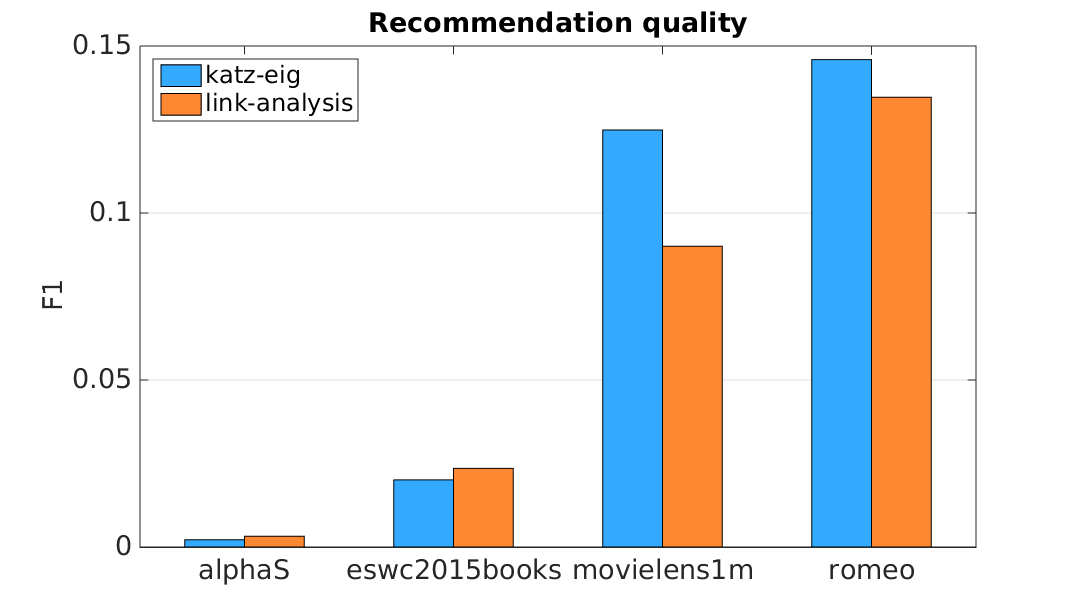
\includegraphics[width=0.9\textwidth]{fig/comp/comp_rec_quality.png}
    \caption{Comparison of the recommendation quality given from the different algorithms, given the optimized parameters specified in \appendixref{app:opt_params}.}
\end{figure}

\begin{figure}[h!]
    \begin{subfigure}[h!]{0.5\textwidth}
        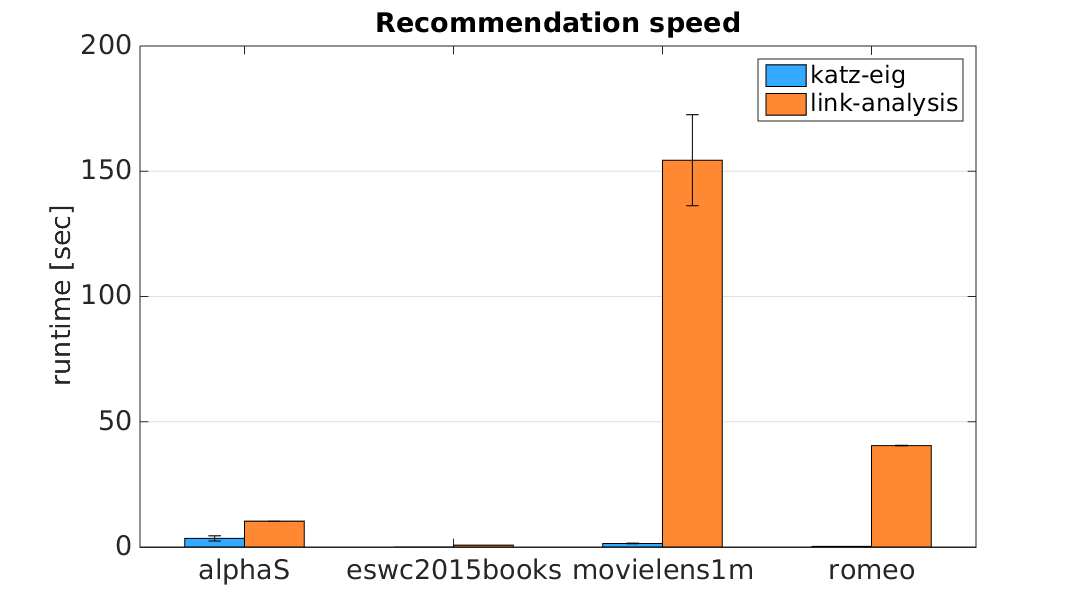
\includegraphics[width=\textwidth]{fig/comp/comp_rec_speed.png}
        \caption{}
        %\label{fig:rec_speed}
    \end{subfigure}
    ~
    \begin{subfigure}[h!]{0.5\textwidth}
        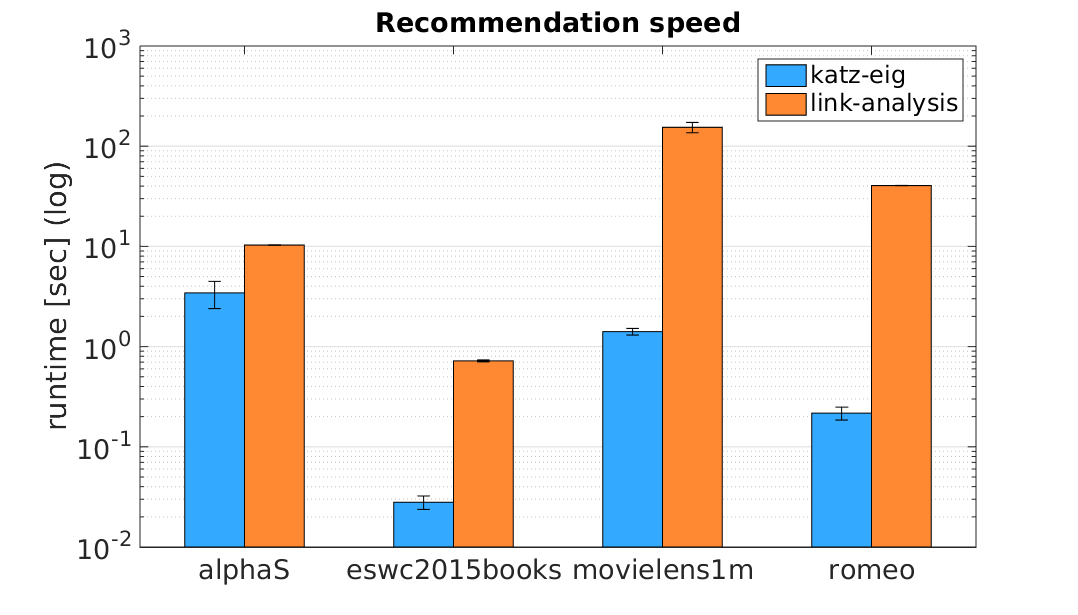
\includegraphics[width=\textwidth]{fig/comp/comp_rec_speed_log.png}
        \caption{}
        %\label{fig:rec_speed_log}
    \end{subfigure}
    \caption{Comparison of the runtime of generating recommendations for the full dataset for the different algorithms. (b) shows the speed with logarithmic y-axis. Both plots include the standard deviation of the 10 runs made.}
\end{figure}

